\chapter{Trajectories}\label{app:trajs}

\begin{table}[h]
\centering
\begin{tabularx}{0.75\textwidth}{|X|X|}
\hline
Parameter & Values \\
\hline
    Deme carrying capacity & $1, 512, 8192, \infty$ \\
    Driver mutation rate & $10^{-6}, 10^{-5}, 10^{-4}$ \\
    Selection coefficient & $0.05, 0.1, 0.2$ \\
    Baseline death rate (non-spatial) & $0.98$ \\
    Baseline death rate (spatial) & $0$ \\
\hline
\end{tabularx}
\caption{Parameters used for the simulations. The deme carrying capacity is
    varied across spatial configurations (boundary growth, invasive glandular,
    gland fission, non-spatial respectively), while other parameter variations
    are common to all simulations.}
\label{tab:traj_params}
\end{table}

\begin{figure}[h]
\centering
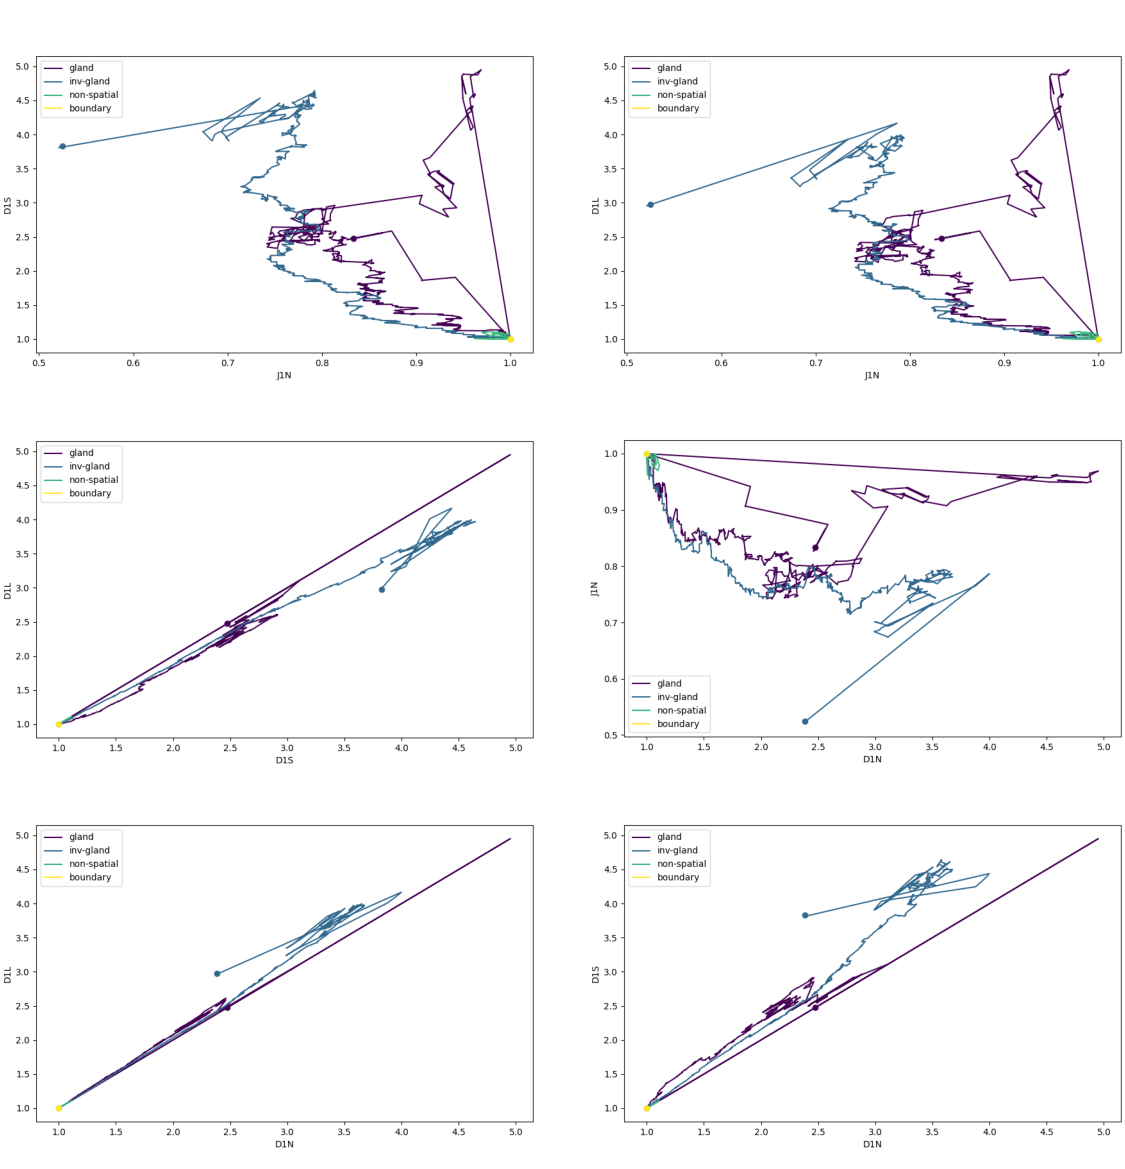
\includegraphics[width=\textwidth]{Chapter_3/figures/1e06005new.pdf}
\caption{Trajectories plotted for the four different spatial configurations for
    the driver mutation rate $\mu=10^{-6}$, and selective coefficient
    $s=0.05$.}
\label{fig:1e06005new}
\end{figure}

\begin{figure}[h]
\centering
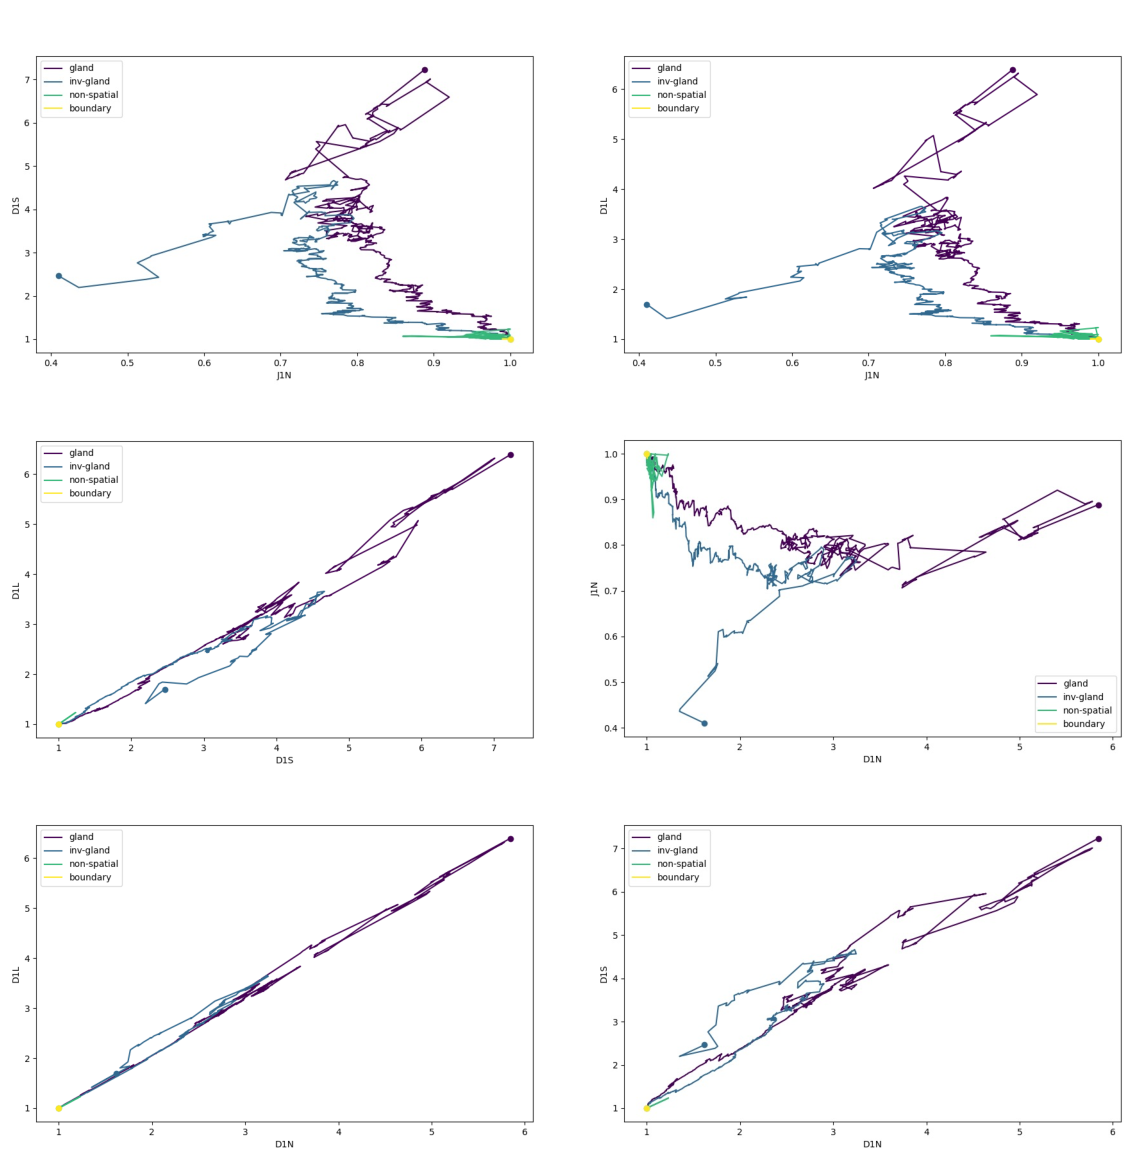
\includegraphics[width=\textwidth]{Chapter_3/figures/1e0601new.pdf}
\caption{Trajectories plotted for the four different spatial configurations for
    the driver mutation rate $\mu=10^{-6}$, and selective coefficient
    $s=0.1$.}
\label{fig:1e0601new}
\end{figure}

\begin{figure}[h]
\centering
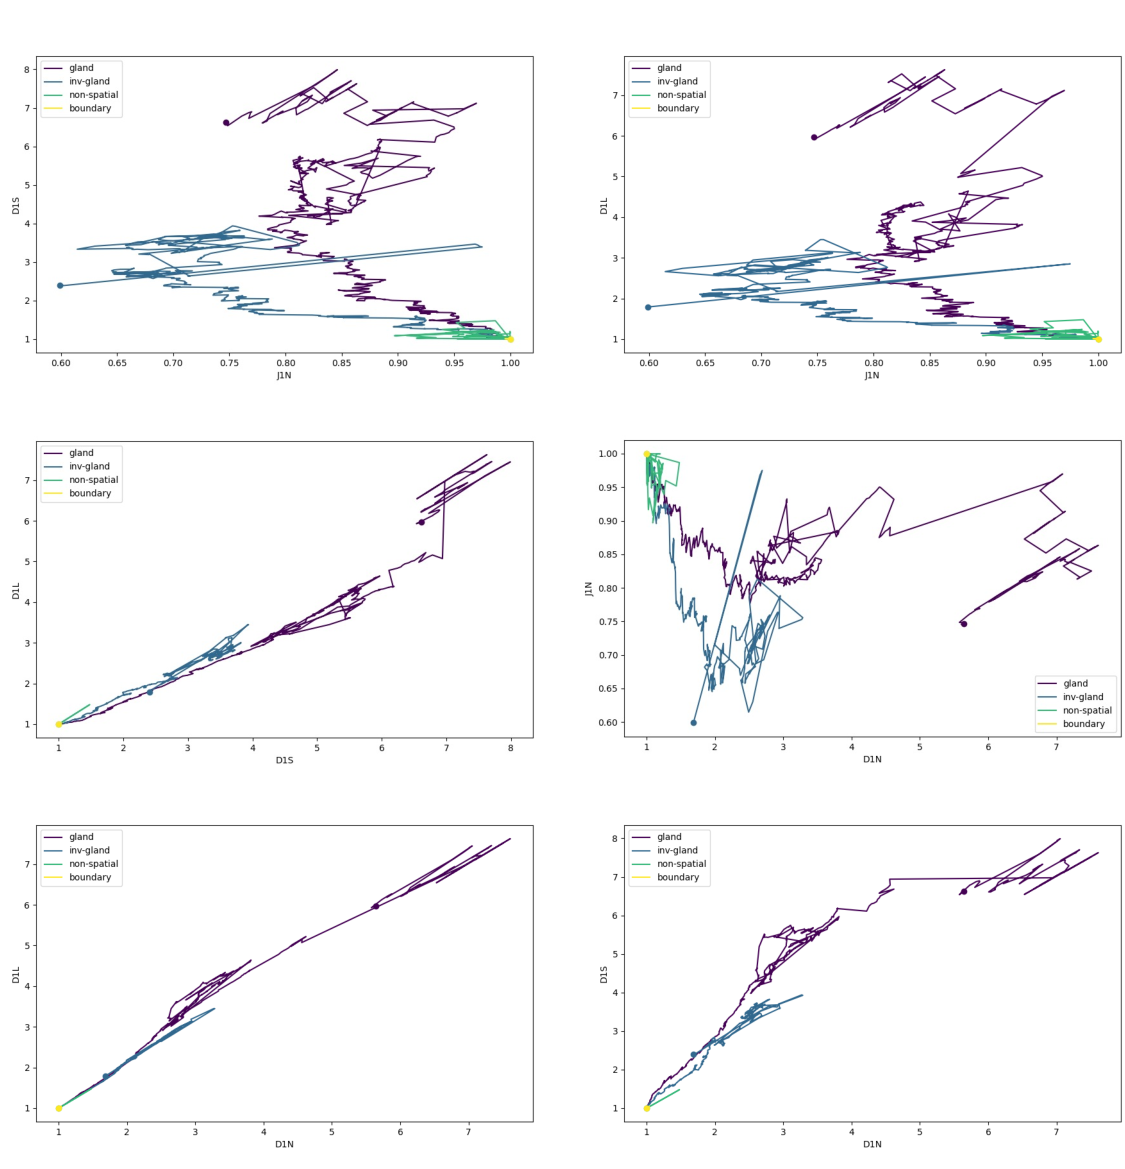
\includegraphics[width=\textwidth]{Chapter_3/figures/1e0602new.pdf}
\caption{Trajectories plotted for the four different spatial configurations for
    the driver mutation rate $\mu=10^{-6}$, and selective coefficient
    $s=0.2$.}
\label{fig:1e0602new}
\end{figure}

\begin{figure}[h]
\centering
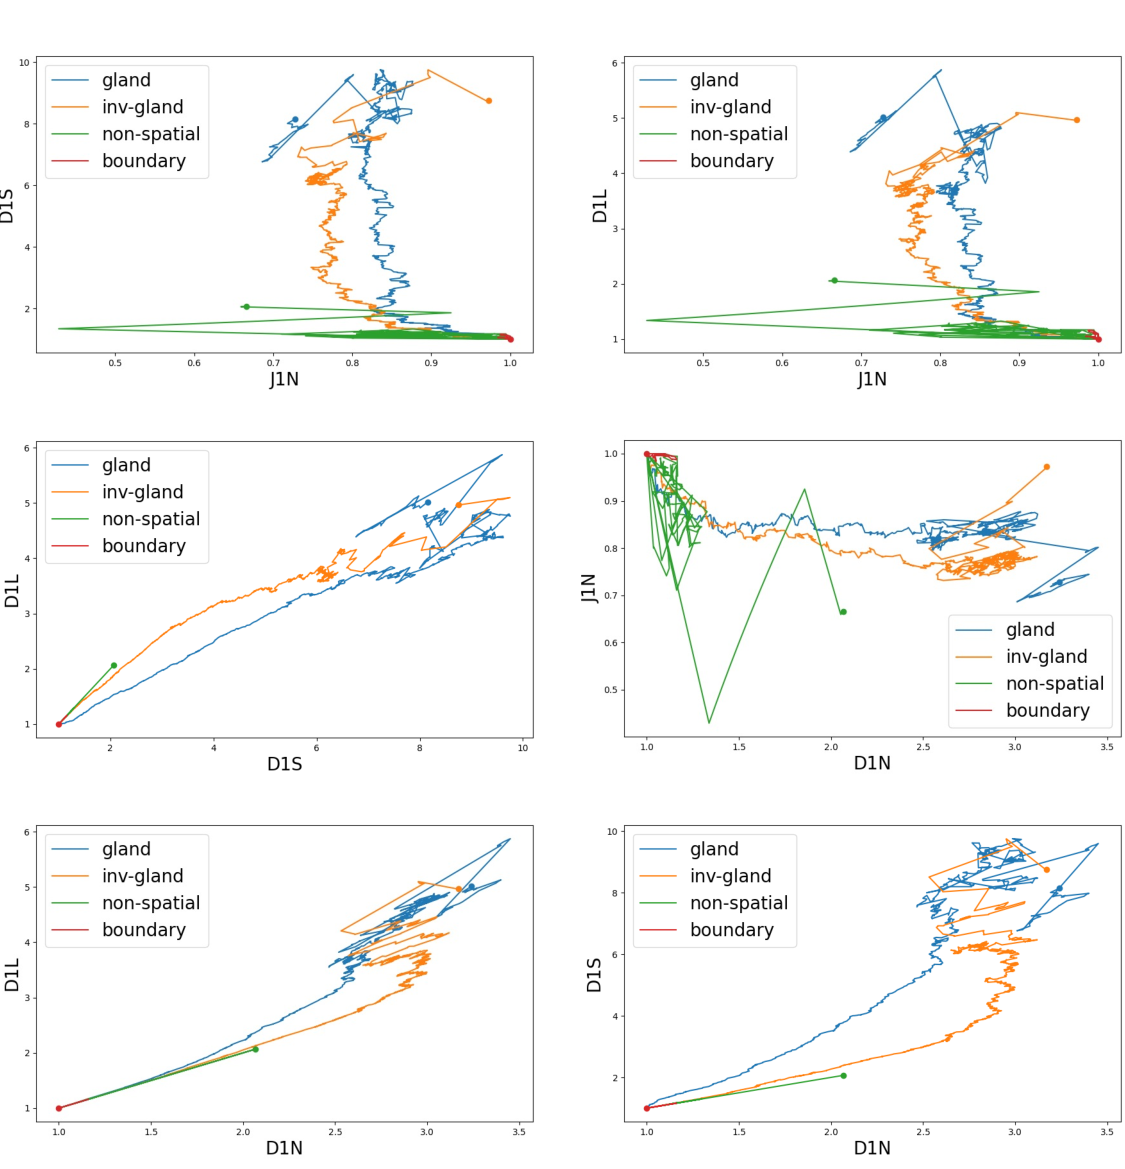
\includegraphics[width=\textwidth]{Chapter_3/figures/1e05005new.pdf}
\caption{Trajectories plotted for the four different spatial configurations for
    the driver mutation rate $\mu=10^{-5}$, and selective coefficient
    $s=0.05$.}
\label{fig:1e05005new}
\end{figure}

\begin{figure}[h]
\centering
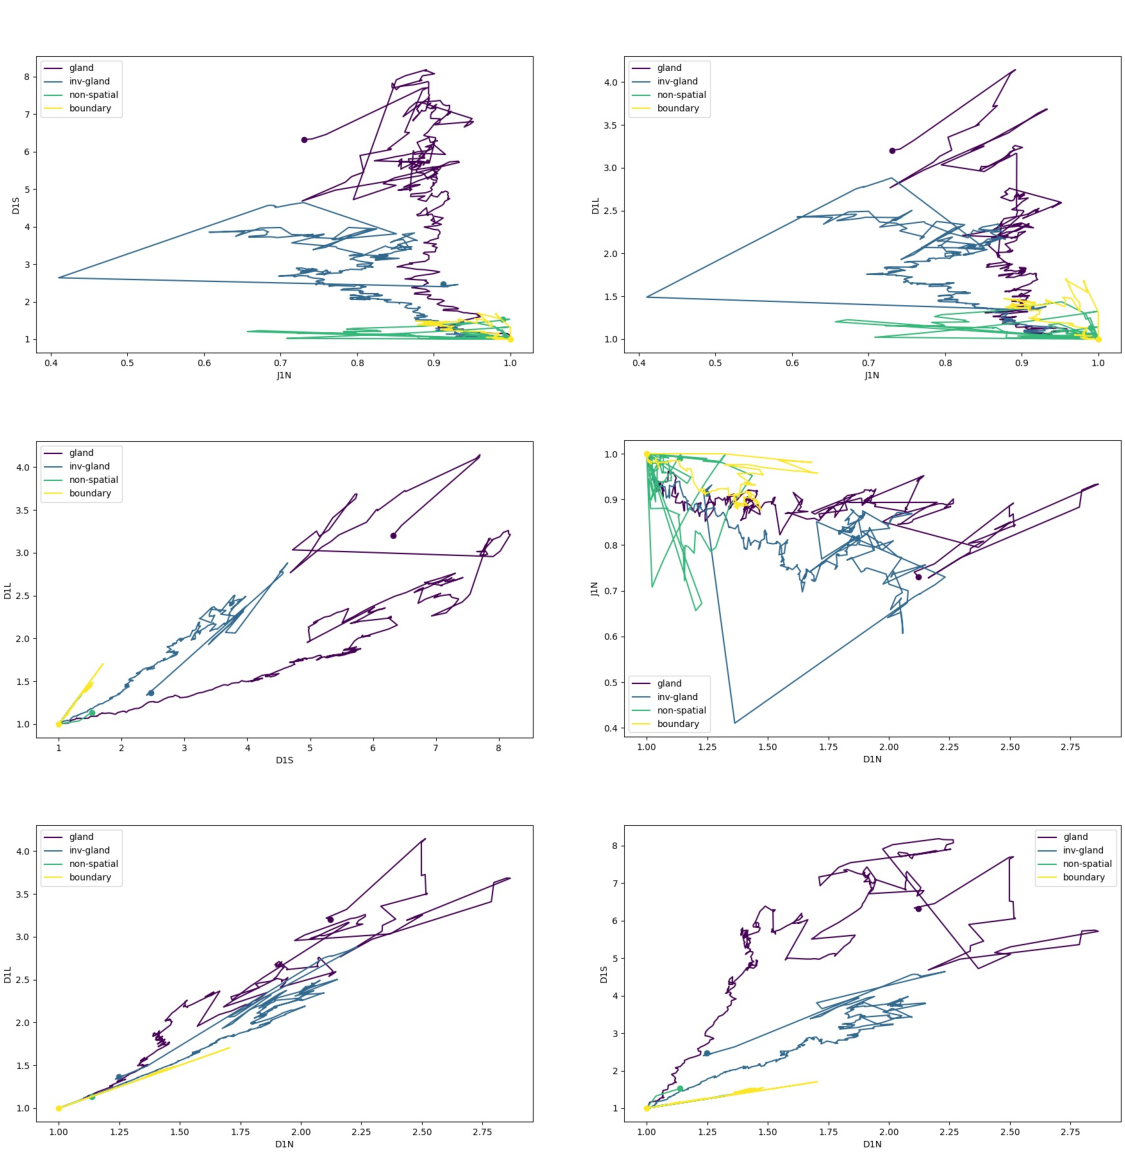
\includegraphics[width=\textwidth]{Chapter_3/figures/1e0502new.pdf}
\caption{Trajectories plotted for the four different spatial configurations for
    the driver mutation rate $\mu=10^{-5}$, and selective coefficient
    $s=0.2$.}
\label{fig:1e0502new}
\end{figure}

\begin{figure}[h]
\centering
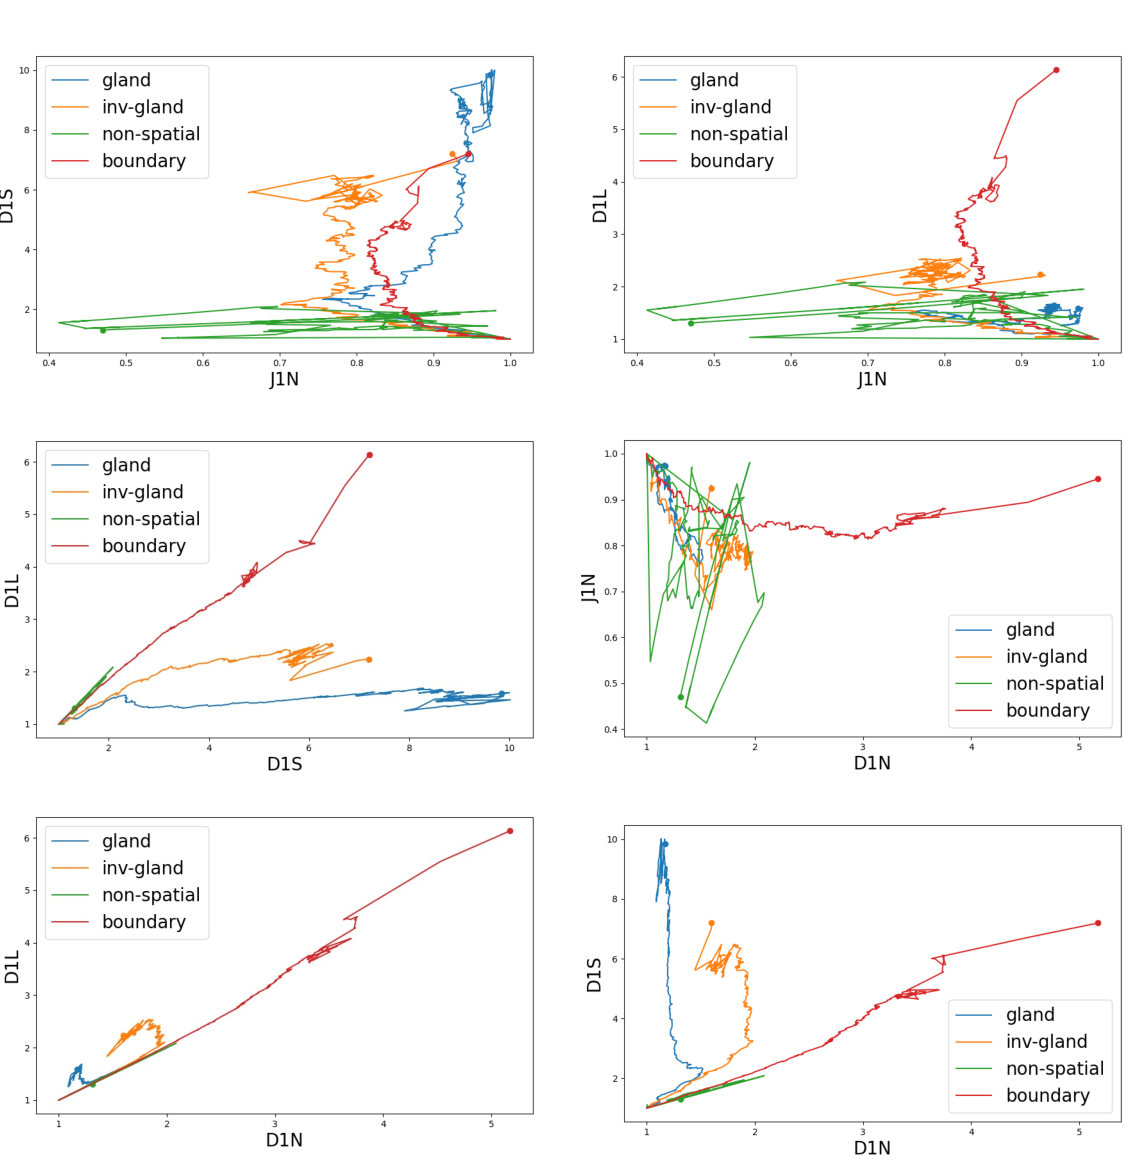
\includegraphics[width=\textwidth]{Chapter_3/figures/1e0401new.pdf}
\caption{Trajectories plotted for the four different spatial configurations for
    the driver mutation rate $\mu=10^{-4}$, and selective coefficient
    $s=0.1$.}
\label{fig:1e0401new}
\end{figure}

\begin{figure}[h]
\centering
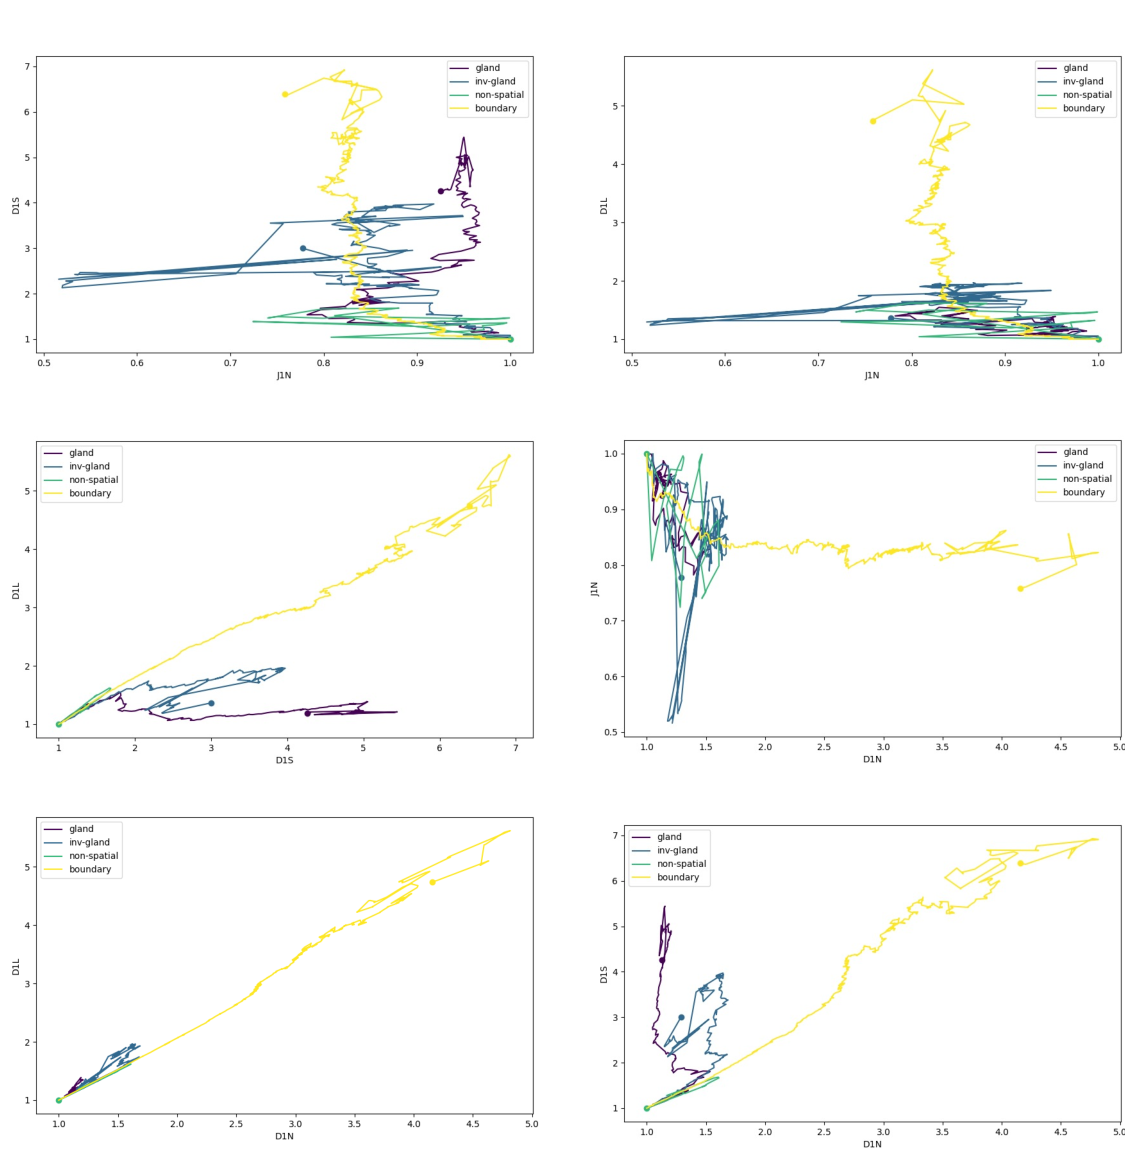
\includegraphics[width=\textwidth]{Chapter_3/figures/1e0402new.pdf}
\caption{Trajectories plotted for the four different spatial configurations for
    the driver mutation rate $\mu=10^{-4}$, and selective coefficient
    $s=0.2$.}
\label{fig:1e0402new}
\end{figure}

